\documentclass[t]{beamer}
\usetheme{Rochester}
\usecolortheme{beaver}
\usepackage{graphicx}
\usepackage{geometry}


\title{MinusMinusEnergy}
\subtitle{Energy Switzerland Challenge}
\author
{M.\,Busenhart \and M.\,Winkler \and M-L.\,Achart \\\and P.\,Wiese \and Y.\,Niedermayr}
\date[BETH 2019]
{BETH - Blockchain for Sustainability, 2019}
\subject{Computer Science}

\logo{ \begin{minipage}{10.2cm}
\includegraphics[height=1.4cm]{BETH.png}\vspace{-0.2cm}\end{minipage} \begin{minipage}{2.5cm}
\includegraphics[height=1.1cm]{swissenergy.png}\vspace{-0.5cm}\end{minipage}}

\begin{document}
  \frame{
    \titlepage
  }
  \begin{frame}
    \frametitle{Concept}
    \begin{figure}
    	 \vskip-2.1cm
    	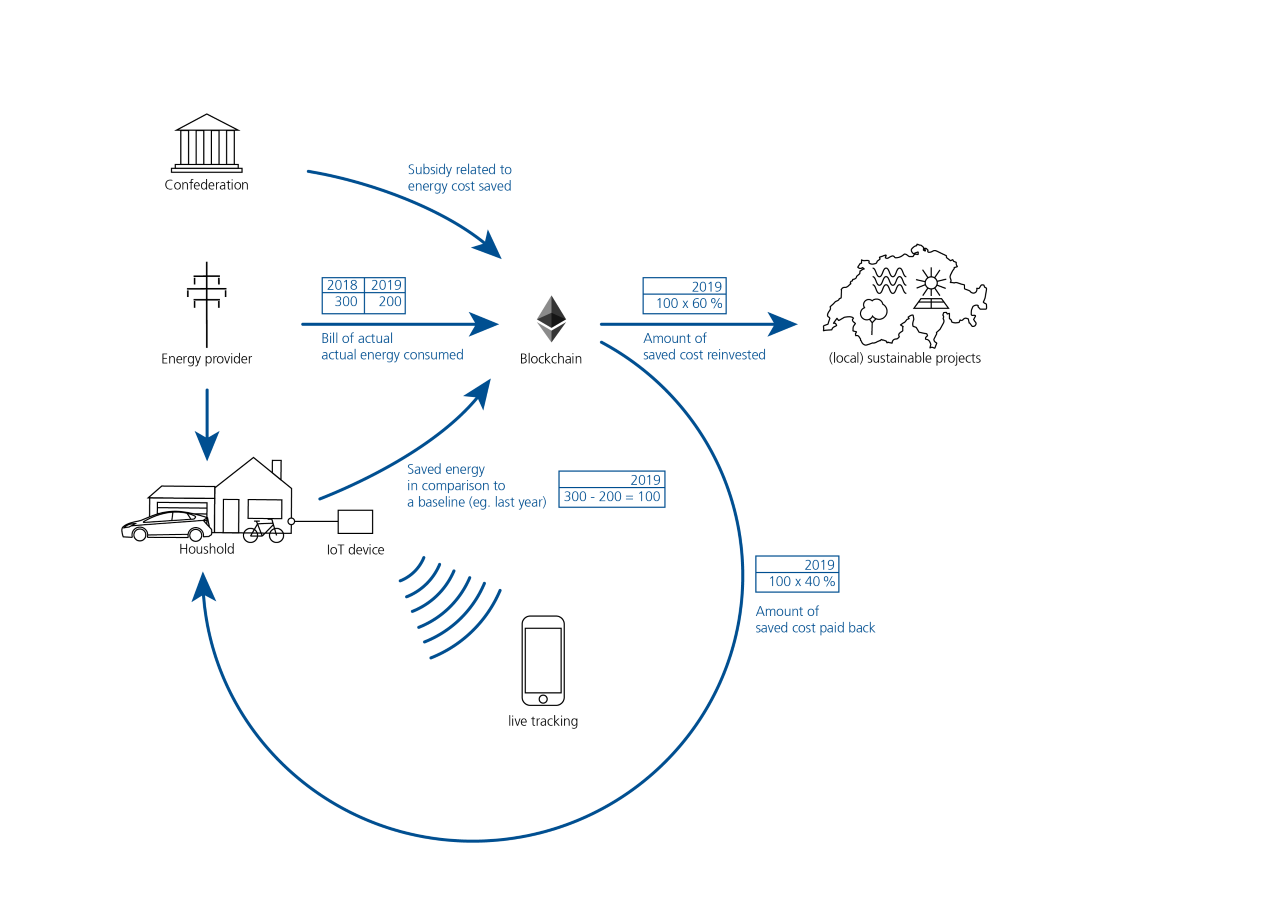
\includegraphics[width=1.25\linewidth]{concept.png}
    \end{figure}
  \end{frame}

  \begin{frame}
		\frametitle{Current Implementation}
		\begin{figure}
			\vskip-1.95cm
			\hskip-2.1cm
			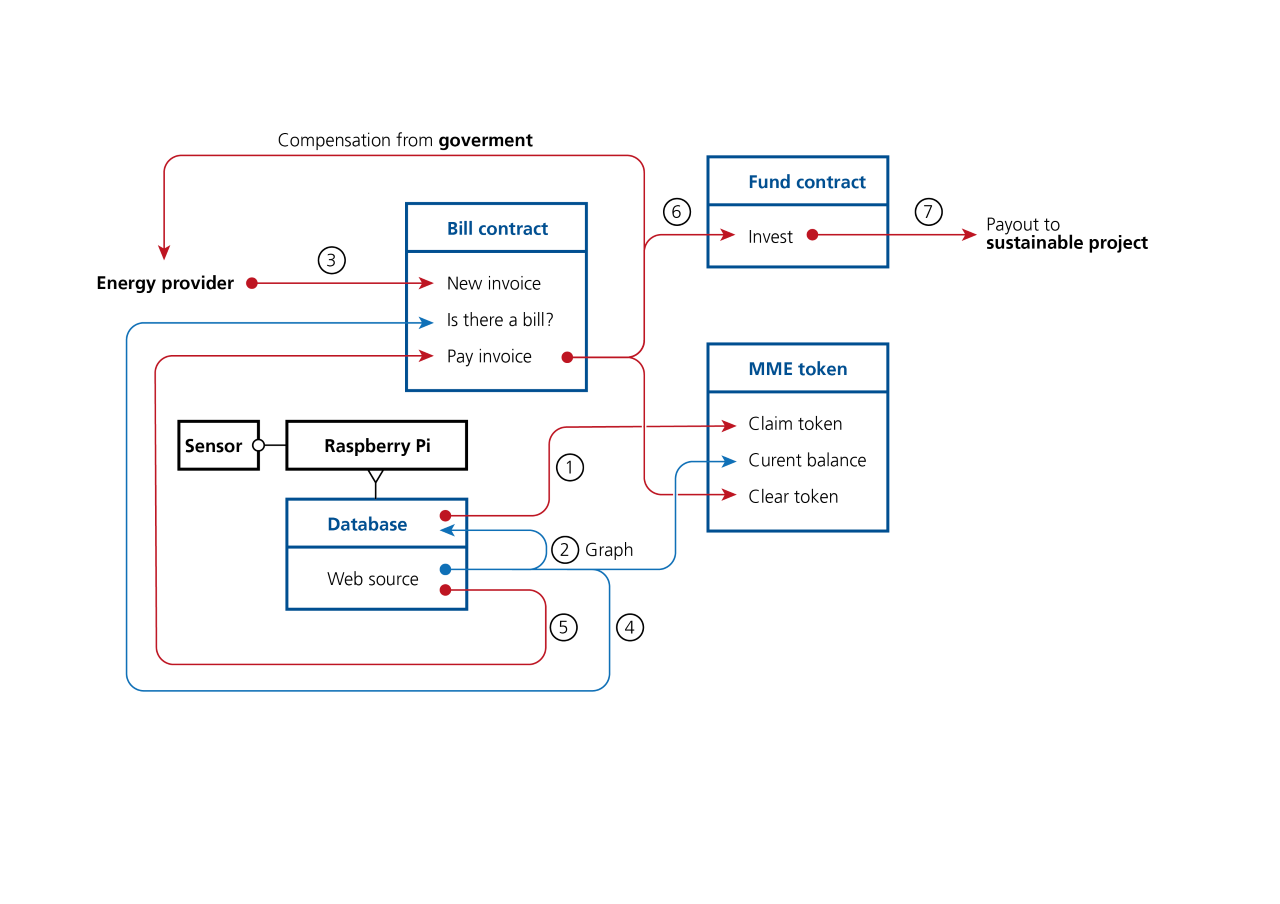
\includegraphics[width=1.2\linewidth]{implementation.png}
		\end{figure}
  \end{frame}

  \begin{frame}[t]
    \frametitle{Disruptive Potential and Further Development}
    \vskip-0.45cm
	\text{Status quo}
	\begin{itemize}
	\item{Simplified \& automated billing thanks to smart contracts}
	\item{Secured data transmission and storage on the Blockchain}
	\item{IoT devices to monitor energy consumption}
	\item{Could be a step toward a decentralized energy grid}    
	\end{itemize}
	\text{Consumer benefits}
	\begin{itemize}
	\item{Relevant visualization and live tracking as incentive}
	\item{Fully interactive reward system: amount and destination of reinvested saved cost is up to the consumer}   
	\item{Consumers gain power and control the amount and destination of reinvested saved cost}
	\item{New paradigm: when the consumer saves energy, he does not only pay less, he also earns more}
	\end{itemize}
    \end{frame}

  \begin{frame}
    \frametitle{Demo}
	\begin{figure}
	\vskip-0.5cm
	    \href{https://github.com/maede97/MinusMinusEnergy/blob/master/doc/demo/fullDemo.gif}{
	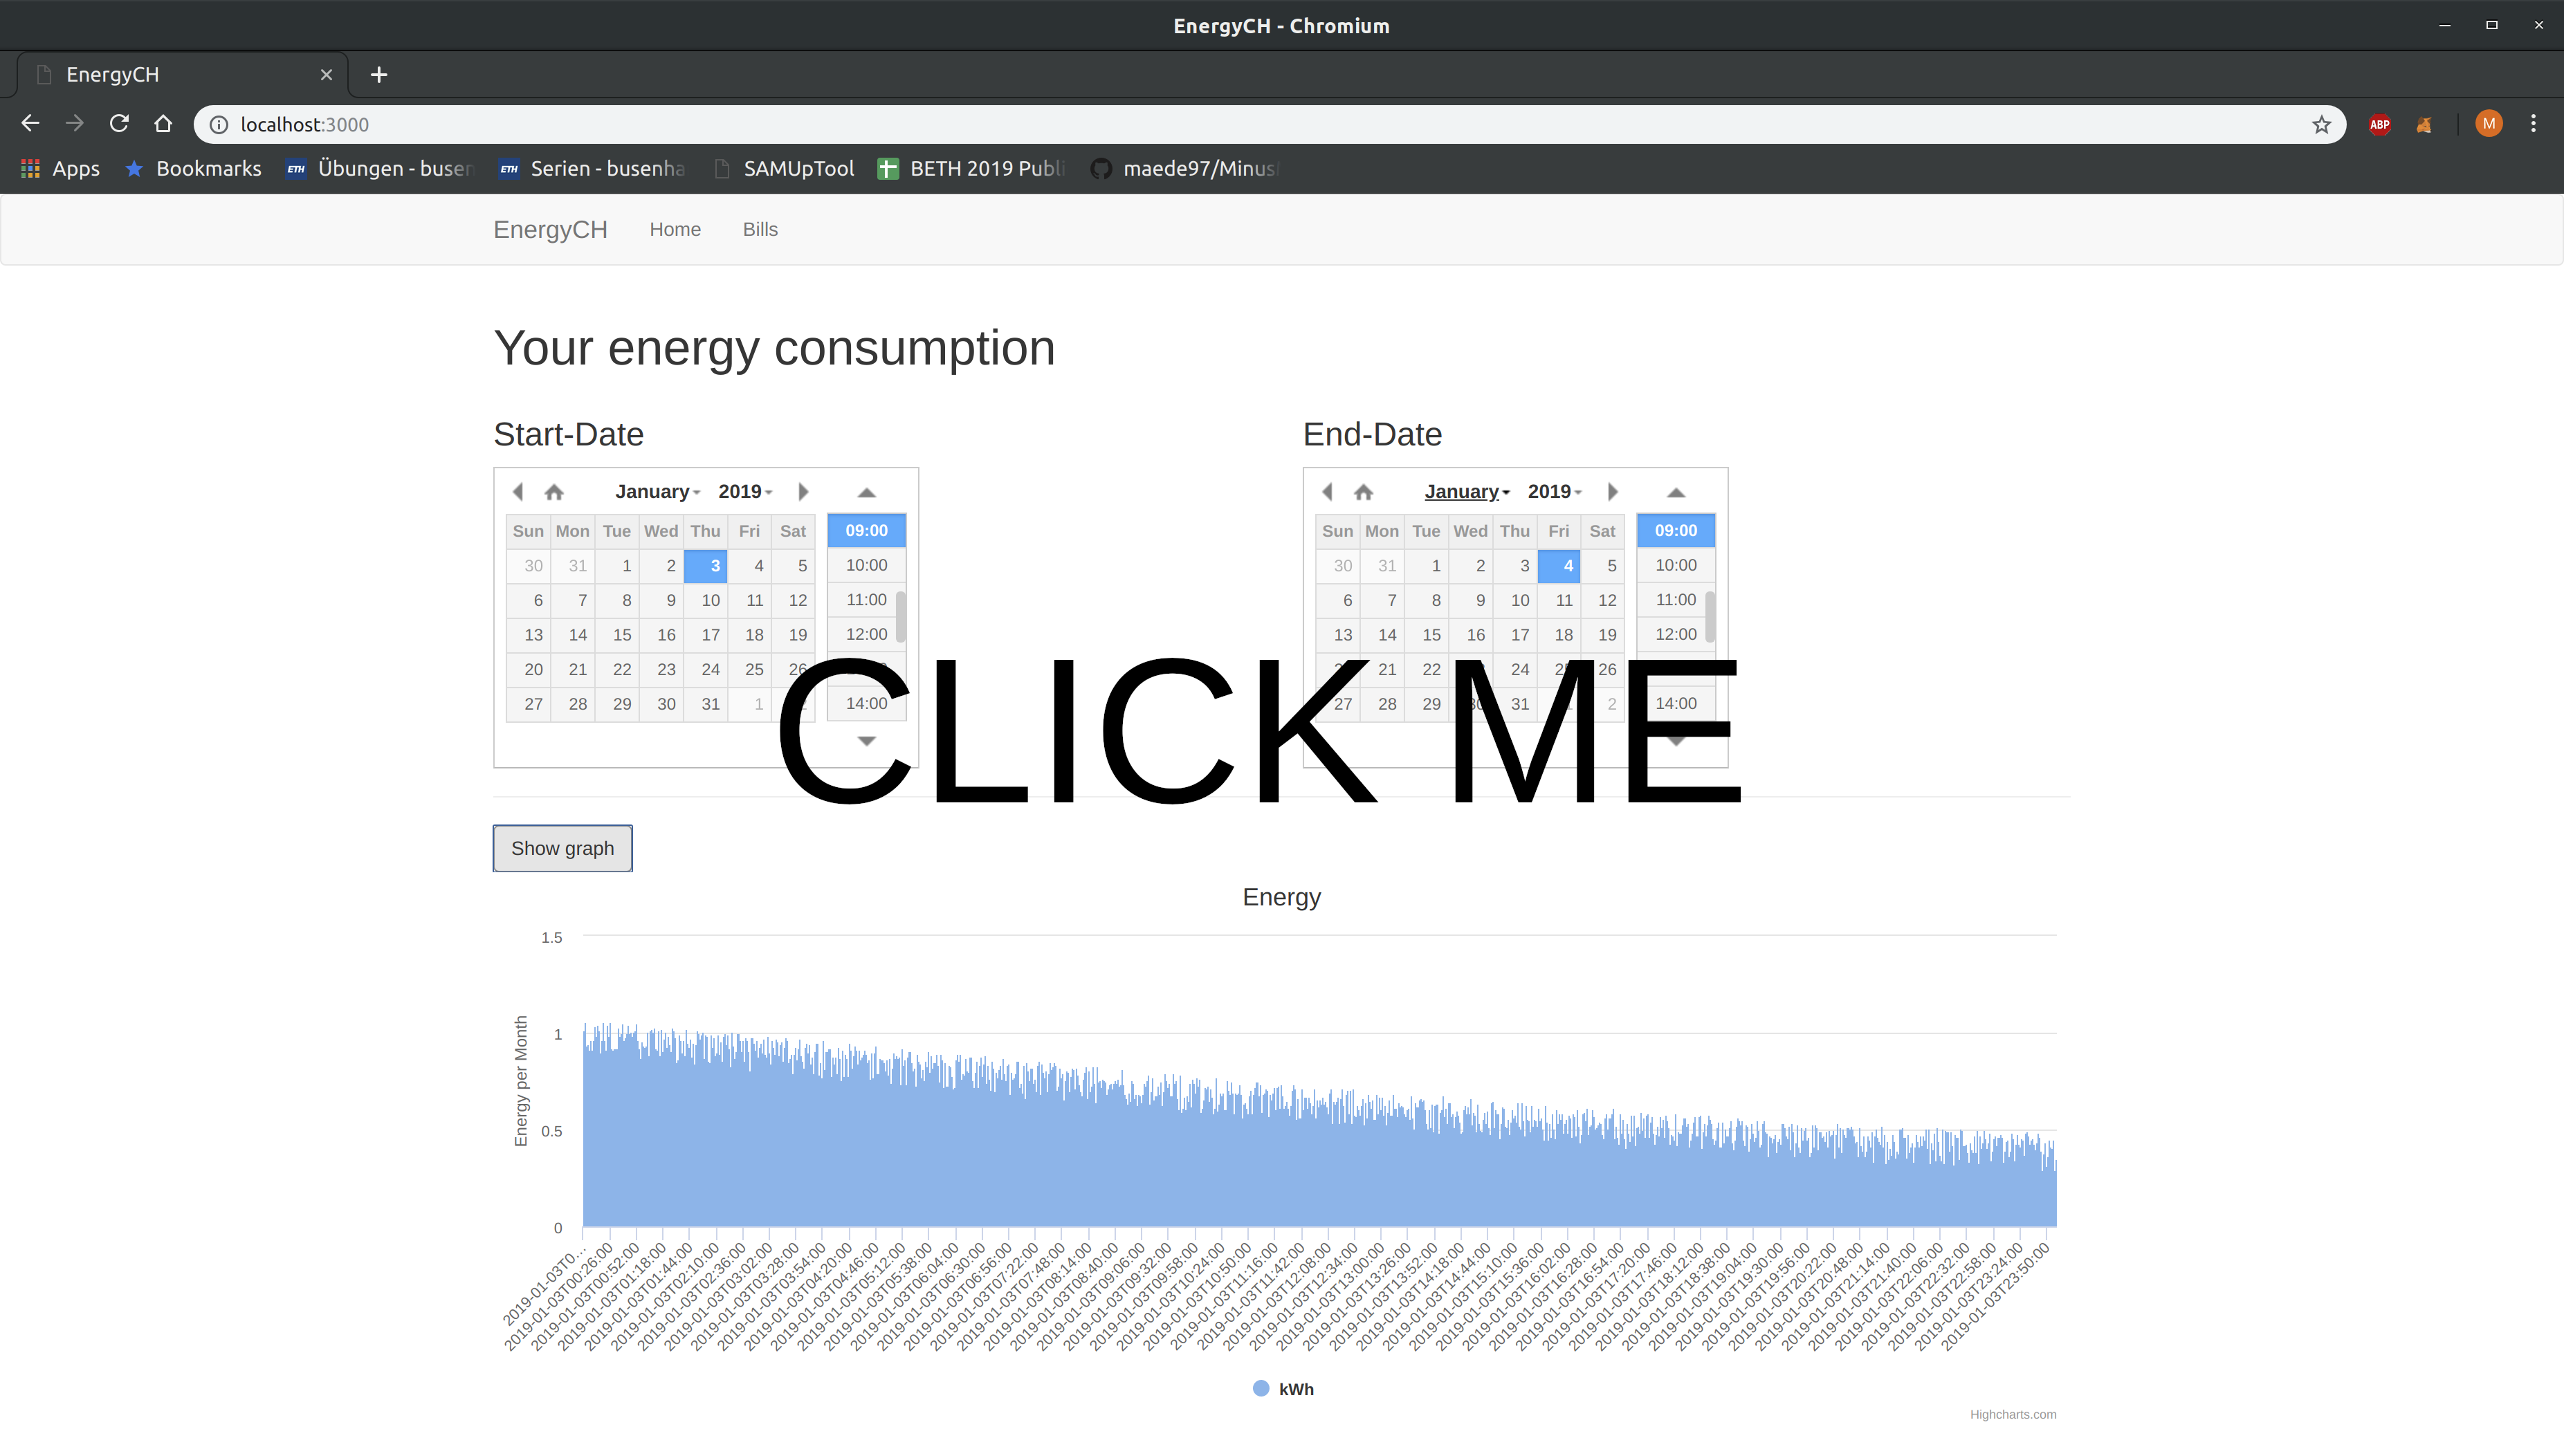
\includegraphics[width=1\linewidth]{demo.png}}
	\end{figure}

  \end{frame}
\end{document}
